\noindent
\begin{tabular}{cc}
\begin{minipage}{0.60\textwidth}
\begin{exerciseS}[Difetto di scia: stima resistenza]
Calcolare la resistenza di un profilo immerso in una corrente stazionaria 
con velocità asintotica ${\bm{V}}_\infty$, sapendo la distribuzione della 
componente di velocità $u(y)$ parallela a ${\bm{V}}_\infty$ a valle del 
profilo e assumendo che:
\begin{itemize}
\item la pressione statica sul contorno del volume di controllo
      sia costante e pari a quella della corrente indisturbata a monte
      del profilo;
\item sul lato superiore e inferiore del volume di controllo
      sia possibile trascurare la componente lungo l'asse $x$ della 
      perturbazione della velocit\`a dovuta alla presenza del profilo:
      $
      \bm{V} = (V_{\infty}+u,v) \simeq (V_{\infty},v).
      $
\end{itemize}
($R = \int_0^{ H}\rho \, u(y) [V_{\infty}-u(y)] dy.$)
\end{exerciseS}
\end{minipage}
&
\begin{minipage}{0.35\textwidth}
   \begin{center}
   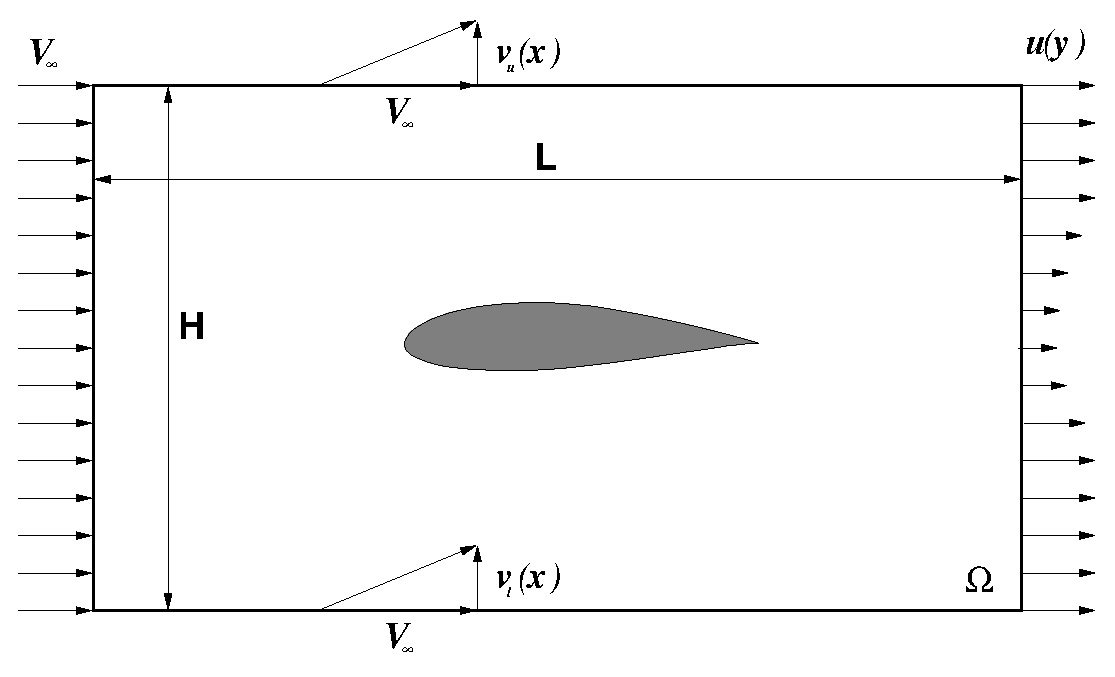
\includegraphics[width=0.90\textwidth]{./fig/airfoil.eps}
   \end{center}
\end{minipage}
\end{tabular}

\vspace{1.0cm}

\sol

\partone
  Bilanci integrali di massa e quantità di moto. Equazioni di equilibrio (equazioni fondamentali della dinamica classica). Principio di azione e reazione. Integrale della normale su una superficie chiusa è identicamente nullo. Esperienza in laboratorio sul \textit{difetto di scia}.

\parttwo
 Vengono scritti i bilanci integrali di massa e quantità di moto, opportunamente semplificati (ipotesi di stazionarietà $\frac{d}{dt} \equiv 0$, densità costante $\rho = \bar{\rho}$, ipotesi sulle condizioni sul bordo esterno del dominio); all'interno dei bilanci si possono riconoscere i termini legati alle azioni scambiate dal fluido con il profilo
 (l'incognita del problema); si sfrutta infine la geometria rettangolare del contorno esterno e le ipotesi su di esso per ottenere una forma ulteriormente semplificata dei bilanci e trovare la soluzione del problema.

\begin{itemize}
  \item Scrittura e semplificazione dei bilanci di massa e quantità di moto.
    \begin{equation}
      \begin{cases}
       \frac{d}{d t} \int_{\Omega} \rho + \oint_{\partial \Omega} \rho \bm{u} \cdot \hat{\bm{n}} = 0 & \qquad \text{(massa)} \\
       \frac{d}{d t} \int_{\Omega} \rho \bm{u} + \oint_{\partial \Omega} \rho \bm{u} \bm{u} \cdot \hat{\bm{n}} +
        \oint_{\partial \Omega} p \hat{\bm{n}} - \oint_{\partial \Omega} \bm{s_n} = 0  
        & \qquad \text{(quantità di moto)}  %\Rb^{ext}
      \end{cases}
    \end{equation}

%Dove $\Rb^{ext}$ è la risultante delle forze esterne che agiscono sul fluido. Nell'ipotesi che non ci siano altre forze esterne agenti sul fluido, se non quelle prodotte dal profilo, la forza $\bm{F}$ esercitata dal fluido sul profilo sarà uguale e contraria a $\Rb^{ext}$. L'incognita del problema è la resistenza del profilo, cioè la componente di $\bm{F}$ nella direzione della velocità asintotica $\Vb_{\infty}$ (in questo caso $F_x$).

Nel problema, il controno del dominio fluido $\partial \Omega$ è costituito dal bordo rettangolare $\gamma_\infty$ lontano dal profilo e dal bordo $\gamma_p$ coincidente con il profilo stesso. La forza $\bm{F}$ agente sul profilo è l'integrale degli sforzi generati dal fluido (uguali e contrari agli sforzi agenti sul fluido) sul contorno del profilo. Inoltre si può fare l'ipotesi di sforzi viscosi nulli e pressione costante sul bordo esterno: l'integrale sul dominio esterno si riduce all'integrale della normale su una superficie chiusa ed è quindi nullo. Si può dunque scrivere:
\begin{equation}
 \oint_{\partial \Omega} (-p \hat{\bm{n}} + \bm{s_n}) = \oint_{\partial \Omega} \bm{t_n} = \underbrace{\oint_{\gamma_p} \bm{t_n}}_{=-\bm{F}} + \underbrace{\oint_{\gamma_\infty} \bm{t_n}}_{=0} = -\bm{F}
\end{equation}

\textit{Osservazione. A differenza di quanto fatto in classe, non
è stata fatta l'ipotesi di fluido non viscoso; il contributo 
all'infinito si annulla con l'ipotesi di pressione costante 
all'infinito e sforzi viscosi trascurabili. Per ritrovarsi con gli appunti, sostituire $\bm{t_n}$ con
$-p\bm{\hat{n}}$}.

Dopo aver fatto l'ipotesi di stazionarietà e aver inserito la definizione di $\bm{F}$ appena data, le equazioni di bilancio possono essere scritte come:
    \begin{equation}
      \begin{cases}
      & \oint_{\partial \Omega} \rho \bm{u} \cdot \hat{\bm{n}} = 0  \\
      & \bm{F} = - \oint_{\partial \Omega} \rho \bm{u} \bm{u} \cdot \hat{\bm{n}} 
      \end{cases}
    \label{eqn:airfoil_bil_int}
    \end{equation}

Il bilancio di quantità di moto può essere scritto esplicitando e
separando le componenti vettoriali.
    \begin{equation}
    \begin{aligned}
       F_x\bm{\hat{x}} + F_y\bm{\hat{y}} 
& = - \oint_{\partial \Omega} \rho (u \bm{x} + v \bm{y}) \bm{u} \cdot \hat{\bm{n}} \\
& =       - \bm{\hat{x}} \oint_{\partial \Omega} \rho u \bm{u} \cdot \hat{\bm{n}} -  \bm{\hat{y}} \oint_{\partial \Omega} \rho v  \bm{u} \cdot \hat{\bm{n}}
    \end{aligned}
    \end{equation}
\item Scrittura delle equazioni di bilancio in componenti (sfruttando la geometria rettangolare del bordo esterno: $\gamma_1$ indica il bordo di sinistra, $\gamma_2$ il bordo inferiore, $\gamma_3$ quello di destra, $\gamma_4$ quello superiore).

\textit{Attenzione: la normale è quella uscente dal dominio fluido. Sul contorno del profilo, la
normale è entrante nel profilo. 
In più: non fare confusione tra azioni del profilo agenti sul fluido e azioni del fluido agenti 
sul profilo!}
  \begin{equation}
     \begin{cases}
      & 0 = \oint_{\partial \Omega} \rho \bm{u} \cdot \hat{\bm{n}} = -\int_{\gamma_1} \rho u
      -\int_{\gamma_2} \rho v +\int_{\gamma_3} \rho u +\int_{\gamma_4} \rho v \\
      & F_x = +\int_{\gamma_1} \rho u^2 +\int_{\gamma_2} \rho u v -\int_{\gamma_3} \rho u^2 -\int_{\gamma_4} \rho u v \\
      & F_y = +\int_{\gamma_1} \rho u v +\int_{\gamma_2} \rho v^2 -\int_{\gamma_3} \rho u v -\int_{\gamma_4} \rho v^2
     \end{cases}
  \end{equation}

\item Ipotesi sulla velocità sui lati orizzontali ($u|_{\gamma_2} = u|_{\gamma_4} = V_\infty$ costante), per poter ulteriormente semplificare il risultato.
   \begin{equation}
     \begin{cases}
        \int_{\gamma_2} \rho v  -\int_{\gamma_4} \rho v = -\int_{\gamma_1} \rho u+\int_{\gamma_3} \rho u\\
       F_x = +\int_{\gamma_1} \rho u^2 -\int_{\gamma_3} \rho u^2 + V_\infty \left[ \int_{\gamma_2} \rho v  -\int_{\gamma_4} \rho v \right]
     \end{cases}
  \end{equation}
E inserendo la prima nella seconda:
\begin{equation}
  \begin{aligned}
       F_x  & = \int_{\gamma_1} \rho u^2 -\int_{\gamma_3} \rho u^2 + V_\infty \left[-\int_{\gamma_1} \rho u+\int_{\gamma_3} \rho u \right] = \\
       & = \int_{\gamma_1} \rho u (u-V_\infty) + \int_{\gamma_3} \rho u (V_\infty-u) = \quad \text{($u|_{\gamma_1} = V_\infty  \Rightarrow $ il primo integrale è nullo)} \\
       & = \int_{\gamma_3} \rho u (V_\infty-u) = \\
       & = \int_{0}^{H} \rho u(y) (V_\infty - u(y)) dy
  \end{aligned}
\label{eqn:difetto_scia}
\end{equation}

\end{itemize}

\noindent
\textbf{Osservazioni.} Tramite la misura del campo di velocità in
galleria è possibile stimare la resistenza del corpo.
Le condizioni di ``aria libera'' e in galleria sono diverse. In generale, in galleria il fluido è confinato dalle pareti di galleria, maggiormente ``vincolato''. Inoltre sulle pareti della galleria esiste una condizione di adesione, $\bm{u}=\bm{0}$: per la conservazione della massa, il rallentamento del fluido in corrispondenza delle pareti della galleria viene compensato da un incremento della velocità nella regione ``più lontana'' dalla parete, rispetto a un corpo in aria libera.
 Per tenere conto di effetti di 
\textbf{bloccaggio} dovuti al confinamento in galleria, è necessario compiere delle correzioni delle misure sperimentali.
Agli effetti di bloccaggio, vanno aggiunti gli effetti di \textbf{galleggiamento} dovuti al gradiente di pressione lungo la galleria, che danno un effetto di resistenza aggiuntiva.
Inoltre è importante che la dimensione del corpo rispetto alla dimensione della galleria non sia né ``troppo grosso'' (per problemi di 'bloccaggio'), né, di solito, ``troppo piccolo'' (per motivi di similitudine; ma sarà argomento di puntate successive del corso...). \'E importante avere in mente la necessità di prestare attenzione a questi aspetti, quando vengono svolte attività sperimentali. Ma questo sarà argomento di altri capitoli o di altri corsi...


